\documentclass[a4paper, 10pt]{article}
\usepackage{appendix}

% \documentclass[a4paper, 10pt]{IEEEtran}

\usepackage[utf8]{inputenc}
\usepackage[T1]{fontenc}
\usepackage[margin=1in]{geometry}
\usepackage{todonotes}
\usepackage{xspace}

\usepackage{booktabs}
\usepackage{colortbl}
\usepackage{tablefootnote}

\usepackage{amsmath}
\usepackage{amssymb}
\usepackage{siunitx}
\usepackage{textcomp}

\usepackage{palatino}

\usepackage{titling}
% \newcommand{\subtitle}[1]{%
%   \posttitle{%

%     \begin{center}\large#1\end{center}
%     \small{\bf (extended abstract)}
%     % \vskip0.5em
%  }%
% }

\PassOptionsToPackage{hyphens}{url}\usepackage[colorlinks,linkcolor=blue,citecolor=blue,urlcolor=blue]{hyperref}

\title{Safety $\neq$ Security \\
\ \\
\large A security assessment of state of the art ASIL-D certified microcontrollers \\
\ \\
\small {\bf (extended abstract)}}
% \subtitle{A security assessment of state of the art ASIL-D certified microcontrollers}

\date{}

\newcommand{\TI}{ASILD1\xspace}
\newcommand{\ST}{ASILD2\xspace}
\newcommand{\NXP}{QM1\xspace}

\newcommand{\unroll}{\texttt{unroll}\xspace}
\newcommand{\auth}{\texttt{auth}\xspace}
\newcommand{\jtag}{JTAG\xspace}

\begin{document}

\maketitle
 
\noindent Microcontroller units (MCU) form the foundation of the modern car. They are used to implement functionalities that can be as simple as opening the window when a button is pressed, or as complicated as Vehicle to Vehicle communications and autonomous driving systems. They can perform non-critical tasks such as controlling the windscreen wipers or extremely critical ones like making sure airbags are deployed in case of emergency. 
 
Over the last two decades the number of electronic controllers in vehicles has increased, making evident the need of ensuring the reliability and safety of these MCUs. 
The ISO 26262 standard -- in particular part 10, Annex. A and part 5, Annex. D -- recognizes the pivotal part that MCUs play in the ecosystem of a vehicle and establishes a framework for the development of safe automotive electronic systems. Part 5 of the standard gives a number of examples of safety mechanisms that can be implemented to mitigate different electric faults that could affect the operation of an electronic system and threaten the safety of the vehicle and passengers. Although these examples and recommendations intend to protect against faults occurring during the normal use of the vehicle, some of these safety measures are also often recommended in the security literature as countermeasures against fault injection (FI) attacks. It is therefore easily taken for granted that MCUs implementing ISO 26262 recommendations (i.e. ASIL chips) are also protected against FI attacks.

Our presentation summarizes our investigations in assessing the effectiveness of the ISO 26262's recommendations to resist against FI. We first compare the resistance to FI of two ASIL-D certified MCUs with a standard (non-ASIL) automotive MCU in a controlled test environment. Next, we explore the risks of FI attacks on ASIL-D chips by disabling the debug interface protection mechanism in our targets. Finally, we discuss the consequences and threats these attacks pose in the automotive context and provide recommendations for mitigating the aforementioned threats.

\section{ISO 26262 and fault injection}

Automotive standards and literature, especially with regards to hardware, primarily deal with safety. In this context, faults are considered as an unintended, abnormal and often random condition caused by the hostile environment in which the hardware resides (e.g. high temperatures, noisy power supply, vibrations, electromagnetic pulses produced by coils, etc). ISO 26262 provides recommendations to mitigate and minimize the impact of these unintentional faults and defines the Automotive Safety Integrity Level (ASIL) risk classification scheme from level A through D. ASIL-D complying MCUs are required to adhere to the most stringent requirements on safety and fault-tolerance in order to achieve absence of unreasonable risk. A fifth level, QM, is defined for parts that only require basic quality management. Fault injection is mentioned in the ISO 26262 only as a method of testing the compliance of the ASIL requirements.  


When shifting to the domain of security, faults are no longer the effect of random and unintended events. They are the result of glitches that are deliberately placed, precisely timed and carefully tuned by an attacker with the purpose of compromising the chip security. FI attacks are in general used to alter the program flow or the processed data. If this is possible, an attacker could, for example, bypass the Secure Boot process by skipping the signature verification and executing unauthenticated code, or recover cryptographic keys using a Differential Fault Analysis (DFA) attack. 

For this work, two methods of injecting faults have been considered: voltage glitching -- a fast variation of the power supply voltage -- and electromagnetic (EM) glitching -- a strong and localized EM pulse. A voltage glitching device is cheap (even less than 100€) but the attack is not localized, as it affects the entire chip, and requires modifying the target board by removing the capacitors. EM glitching on the other hand requires no modifications on the board and the glitches are local (i.e. they affect a small area of the chip) but the equipment required is far more expensive. 

%During a FI campaign, most of the active time is spent tuning parameters. The parameter of importance for both methods of glitching is the glitch offset, relative to a fixed trigger point. For power glitching, the other two parameters to consider are the glitch voltage, which is the amount by which the voltage should be dropped, and the glitch length, which is the amount of time this lowered voltage should be maintained. For EM glitching the relative strength of the pulse has to be tuned, along with the position in all three dimensions. Additionally, the size and polarity of the coil can be of importance.

\section{Targets}
To investigate the effectiveness of safety mechanisms as countermeasures against fault injection attacks, two ASIL-D certified MCUs that implement these countermeasures have been selected, from two different % and well-known 
manufacturers. Although we are convinced that we would have obtained similar results with any other ASIL-D MCU in the market, we omit the chip models because we are still in the process of disclosing the findings to the manufacturers in a coordinated manner. The first target, codename \TI, implements an ARM Cortex-R4 core and the second target, codename \ST, a PowerPC e200. These two targets were selected because they represent two of the most prevalent architectures in the safety electronic industry. For reference, a non-ASIL target has been chosen, code-named \NXP. This target implements an ARM Cortex-M0 and can be used for applications which require only the basic QM rating.

From all the safety mechanisms implemented in ASIL-D MCUs, we are only interested in investigating the ones that have an effect on transient faults as they could also mitigate the glitches used by an FI attacker. In both selected targets these mechanisms include a dual core CPU in lockstep configuration (or `Simple Time Redundancy with Comparison') and memories with error correction codes (ECC) and parity bits, as recommended by ISO 26262 part 5. %Lockstep works by running two executions in parallel with a slight delay, and comparing the outcome of the execution afterwards. ECC utilize additional bits to calculate checksums. A parity bit is the simplest version of an ECC scheme and can merely detect bit flips that result in a , more elaborate schemes can detect multiple bit upsets and correct them as well, depending on the amount bits and scheme used.


\section{Characterization}
\label{sec:char}

% \begin{table*}[tb]
% \centering
% \begin{tabular}{@{}l cc cc cc @{}}
% \toprule
%          & \multicolumn{2}{c}{\unroll}  & \multicolumn{2}{c}{\auth}        & \jtag       \\
%           \cmidrule(lr){2-3}            \cmidrule(lr){4-5}                   \cmidrule(l){6-6}      
%          & Power                        & EM                               & Power                        & EM                              & Power       \\
% \midrule
% \NXP     & \cellcolor{gray!25}          & \cellcolor{gray!25}              & \cellcolor{gray!25}          & \cellcolor{gray!25}             & \cellcolor{red!25}X  \\
% \TI      & \cellcolor{red!25}X & \cellcolor{red!25}X     & \cellcolor{red!25}X & \cellcolor{red!25}X    & \cellcolor{yellow!25}X  \\
% \ST      & \cellcolor{green!25}X & \cellcolor{red!25}X     &  \cellcolor{gray!25}         & \cellcolor{red!25}X    &  \cellcolor{gray!25}  \\
% \bottomrule
% \end{tabular}
% \caption{An overview of the different experiments} 
% \label{tab:experiments}
% \end{table*}

\begin{table}[tb]
\centering
\begin{tabular}{@{}l cc cc cc @{}}
\toprule
         & \multicolumn{2}{c}{\unroll}  
         & \multicolumn{2}{c}{\auth}        
         & \multicolumn{1}{c}{\jtag}       \\
           
           \cmidrule(lr){2-3}  \cmidrule(lr){4-5}  \cmidrule(l){6-6}      
           % \cmidrule(lr){2-5}  \cmidrule(lr){6-9}  \cmidrule(l){10-11}      
         
         & \multicolumn{1}{c}{Power}                        & \multicolumn{1}{c}{EM}  
         & \multicolumn{1}{c}{Power}                        & \multicolumn{1}{c}{EM}                              
         & \multicolumn{1}{c}{Power}       \\
           
           % \cmidrule(lr){2-3}  \cmidrule(lr){4-5}  \cmidrule(l){6-7}      
           % \cmidrule(lr){8-9}  \cmidrule(l){10-11}     
        
         % & s & u 
         % & s & u 
         % & s & u 
         % & s & u 
         % & s & u \\

           %\cmidrule(lr){2-3}  \cmidrule(lr){4-5}  \cmidrule(l){6-7}      
           %\cmidrule(lr){8-9}  \cmidrule(l){10-11}    
        \midrule
\NXP      
         & \cellcolor{gray!0}TBD       %& \cellcolor{gray!0}TBD  
         & \cellcolor{gray!0}TBD       %& \cellcolor{gray!0}TBD
         & \cellcolor{gray!0}TBD       %& \cellcolor{gray!0}TBD        
         & \cellcolor{gray!0}TBD       %& \cellcolor{gray!0}TBD
         & \cellcolor{red!0}80\%       %& \cellcolor{red!0}\textasteriskcentered            
         \\
\TI      & \cellcolor{red!0}87\%       %& \cellcolor{red!0}100\%     
         & \cellcolor{red!0}0.2\%      %& \cellcolor{red!0}100\%           
         & \cellcolor{red!0}60\%       %& \cellcolor{red!0}100\%    
         & \cellcolor{red!0}0.2\%      %& \cellcolor{red!0}100\%           
         & \cellcolor{yellow!0}1.3\%  %& \cellcolor{yellow!0}23\%           
         \\
\ST 
         & \cellcolor{green!0}0\% %& \cellcolor{green!0}\textasteriskcentered    
         & \cellcolor{red!0}2.6\%      %& \cellcolor{red!0}100\%    
         & \cellcolor{gray!0}\textasciitilde          %& \cellcolor{gray!0}  
         & \cellcolor{red!0}12\%       %& \cellcolor{red!0}100\%  
         & \cellcolor{gray!0}\textasciitilde          %& \cellcolor{gray!0}              
         \\
\bottomrule
\end{tabular}
\caption{An overview of the success rates of teh different experiments} 
\label{tab:experiments}
\end{table}





The general effectiveness of these safety mechanisms to prevent FI has been investigated in a characterization setup which involves two experiments in a controlled environment. In both experiments a customized trigger signal is generated by the firmware on the target to indicate to the setup when to inject a glitch. The parameters of the glitches (e.g. position, length, power) are randomly changed during the experiments in order to find the most effective values.

In the first experiment, \unroll, a sequence of increment instructions is performed on the same CPU register. This should produce a predictable final value in the counter register. The final value of the register is sent over a serial connection at the end of the sequence together with the internal state of the MCU and the fault detectors. A successful glitch affects the register value by altering the content of the register itself or by changing the code flow and skipping some increment instructions, without triggering the fault detectors.

\unroll is one of the most basic experiments that can be performed and a good starting point for characterizing MCUs. The goal of the test is to confirm that the target is sensitive to FI. If successful glitches are found, additional experimentation should be done involving more realistic scenarios. The additional experiment chosen in this work is referred to throughout as \auth. In this experiment an \texttt{if}-statement determines the program flow, simulating a situation where some authentication check is performed. A successful glitch affects the \texttt{if}-statement in such a way that the unintended branch is executed.

The first two columns of \autoref{tab:experiments} show the results of the two different experiments on the different targets. These percentages represent the success rates obtained after finding and using the most effective glitch parameters (i.e. the counter register was affected or the desired execution branch was reached). Note that while for some parameters a certain percentage of these glitches triggered the fault detectors, the parameters that were used to obtain the percentages shown in \autoref{tab:experiments} had none of the glitches detected. The only exception here is the \TI \jtag result, which will be addressed in the next section. 

The primary conclusion to be drawn from these characterization experiments is that it is possible to find glitch parameters, for both \TI and \ST, which result in a relatively high rate of successful and undetected glitches. Contrary to expectations, all the previous experiments used a single glitch to inject the same fault in both lockstep CPUs. Moreover, when using two glitches separated the same number of clock cycles as the separation of the lockstep execution pipelines, the success rate decreases drastically.

For \TI, both voltage and EM glitches were used with a 60\% of success rate in \textasciitilde9,000 voltage glitching attempts and a 0.2\% of success rate in \textasciitilde8,400 EM glitching attempts, respectively. For \ST, due to the on-chip voltage regulator and special internal power distribution, only EM glitching was successful for 2.6\% of the \textasciitilde21,000 attempts. Note that the EM glitching percentages in both experiments are lower because these tests require more time to find the optimal position of the coils used for injecting the EM pulses. Due to time limitations, it was not possible to narrow down the parameters to find the optimal glitch. It is reasonable to expect that, with the optimal glitch configuration, the success rate would be at least as high as in the voltage glitch experiments.

%This is a generic observation generic to any FI experiment. I think that regarding this point, it would be interesting to mention the double exponential shape which indicates the presence of a second CPU. But this is too much detail for the abstract%

%Other observations made during the characterization stage are the fact that many parameters have some relationship with other parameters. \todo{pictures or nah?} In the case of power, glitch length and glitch voltage show a relationship in the observed effect. Glitch length also shares a relationship with glitch offset. In the case of EM glitching, the power of the pulse is related to the spatial point from which the pulse is shot. Also note that most parameters influence the observed effect by themselves.\todo{weird final sentence}%

% 		short explanation of setup 1 and 2
% 		overview of results of both setups
% 		picture of unroll (curve) or auth (offset relationship)
% 		picture of EM spatial effect
% 		summary of observations
% 		explanation of observations? maybe too much detail
% 		summary of explanationnations

% 		mention it was unexpected that lockstep can be 'ignored'

\section{Breaking JTAG protection}
\label{sec:jtag}
%	picture of differential traces?
%	1 page

%		explanation of addition of side channel analysis
%		words on why countermeasures dont or barely play a role?\\
		

Previous experiments show that is possible to use FI on ASIL-D MCUs to affect the code execution flow and bypass instructions, even if lockstep CPUs and ECC protected memories are used. These experiments were run in a white-box manner in a controlled environment with full control over the software, including the trigger. Real attacks are normally executed in a black-box manner where the attacker has no control over the CPU and no access to the code. In order to have a better understanding of the risks that FI attacks pose on a real application, we prepare a new FI experiment in a non-controlled environment. As the debug interface access is one of the first assets that an attacker tries to obtain, we assess the resistance of the debug interface protection mechanism against FI attacks.

Most modern MCUs have a permanent protection for closing the debug interfaces. This protection is usually enabled at the end of the manufacturing process of the embedded system in order to protect the firmware contained in the MCU. It is a common practice for many semiconductor manufacturers to implement this debug interface protection in the ROM code executed at boot time, before the application firmware is executed. This ROM usually reads the protection configuration from an OTP memory section or a Flash word and configures the registers of the debug interface module accordingly. An attacker using FI to bypass the configuration read or the debug module configuration stage effectively unlocks the debug interface on a protected device, which is regarded here as a successful glitch. 

Because the ROM is immutable, the boot process firmware cannot be modified to generate a trigger for the glitching device. The attacker has to rely purely on measuring the time after releasing the reset to inject the glitch. Some MCU datasheets give some general information about the boot process, but the precise timing information required to trigger the glitch is typically missing. Additionally, time between release of the reset and the area in which a glitch is needed is typically not time-constant. If ROM code is obtainable, the attacker can reverse it to determine exactly when the debug protection mechanism is configured and when to inject the fault, but normally the ROM is proprietary and not accessible. Injecting glitches randomly at boot time is possible when the boot-up time is short -- less than \textasciitilde10,000 clock cycles from the reset to the user application execution -- but is not feasible when more time is required, as is the case with the tested targets. As an alternative, side channel analysis can be used to determine when the debug protection mechanism is configured. We observe that by comparing the power consumption traces of the boot process in a protected and an unprotected chip, an attacker can find the moment in time where the debug interface protection is enabled and get the timing information needed for injecting a glitch. Figure~\ref{fig:jtag2-trace2} shows this power difference in target \TI.

\begin{figure*}[h]
  \centering
  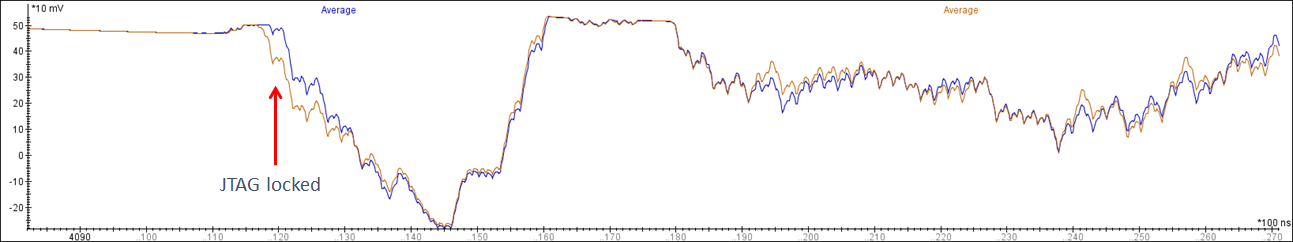
\includegraphics[width=\textwidth]{tms570-DPA-jtag}
  \caption{Difference between locked chip (brown) and unlocked chip (blue) for \TI}
  \label{fig:jtag2-trace2}
\end{figure*}

A full attack -- power analysis to find the timing and injecting voltage glitches to unprotect the JTAG debug interface -- is run on targets \TI and \NXP. From all the debug interfaces supported by our targets -- JTAG, SWD, UART and CAN -- we choose attacking JTAG because it is the most common one. Both experiments succeeded in disabling the JTAG protection with a single glitch. On the \TI target, \textasciitilde677,000 glitches were injected in total for a broad range of different glitch parameters. After tuning the process, 35,200 glitches with the optimal parameters were injected. 1.3\% of the attempts succeeded to unprotect the JTAG without triggering any lockstep or memory faults. An additional 1.2\% of the glitches succeeded to unprotect the JTAG but were detected by the safety mechanisms. Finally, 3.2\% of the attempts had no apparent effects other than triggering the fault detector mechanisms.   %, as shown in \autoref{tab:experiments}\todo{the absolute number of glitches for broad parameter settings, but then the percentages of a very specific set of fixed parameters, might be confusing}. An additional 3.2\% of the glitches were not successful, yet still detected, bringing the amount of successful glitches that were not detected to 23\%, relative to the glitches that were detected. \todo{are all these percentages and categories too confusing?}%
This means that target \TI can be unprotected in less than one minute and half approximately. For comparison purposes, we repeated the experiment on the target \NXP with \textasciitilde89,000 glitching attempts in total. Using the optimal glitch parameters, 80\% of the \textasciitilde10,800 attempts succeeded in unprotecting the JTAG interface, which means that an attack take less than 5 seconds to succeed.

It is not possible to directly compare results on \TI and \NXP because both chips are implemented with different technologies which could have different sensitivity to FI attacks. However, the big gap between success rates indicates that some of the ASIL-D safety mechanisms could slightly mitigate the FI attacks, but cannot fully prevent them.


\section{Security consequences}

The experiments described in \autoref{sec:char} and \autoref{sec:jtag} prove that FI attacks can bypass the detection mechanisms outlined above in state of the art ASIL-D certified MCUs. Although the safety mechanisms detect some glitches, they are not good enough to prevent a FI attack.

The fact that it is possible to bypass instructions or execute an unintended branch means that the integrity of the code execution cannot be assured. Any security feature enabled and any check executed in the software can be manipulated by the attacker as previous step toward gaining access to assets. Various assets can be targeted, depending on the attacker profile and the attack scenario. The most common assets include firmware extraction, firmware manipulation, runtime control and access to debug interfaces.

The firmware contained in MCUs is usually the most valuable secret of Tier1 manufacturers and OEMs. The firmware implements those functionalities that add value to the product and differentiate the brand from the competitors. Taking for example a brake controller assistant or an autonomous driving system, there are thousands of hours invested in research and development of the perfect algorithms for stopping the car safely or driving it autonomously through the city. A competitor extracting the software of an ECU would have access to those proprietary technologies and could copy them, or use them to improve their own technology and gain an unfair competitive edge. Extracting the software can also be an intermediate step for achieving a bigger objective. An attacker could reverse engineer the extracted software to understand its operation and find a vulnerability. This has been done several times in the past when researchers reversed the firmware of the remote key entry systems and immobilizers. Vulnerabilities in the cryptographic algorithms were found, which allowed cloning the keys to open and start the car. Similarly, researchers reversed the extracted software to find remotely exploitable vulnerabilities which gave control of the car without even needing physical access to it.

Modifying the firmware is another common objective of attackers. Typically this attacker profile includes car tuners who seek to modify the performance of their vehicles by altering the software. These persons normally are not aware of the risk that those unlawful modifications could pose to their and others lives. A less common profile could be subjects that are purposely looking to inflict damage in the vehicle or to its occupants by the means of sabotage. In both cases, the possibility of altering the MCU firmware without any tamper evidence is appealing and it should be prevented by the manufacturers.

Runtime control and access to debug interfaces are usually intermediate steps that are necessary for gaining any of the assets mentioned. For example, the attack executed in \autoref{sec:jtag} for gaining JTAG access could be used to extract and modify the firmware in the MCU. An additional benefit of gaining runtime control or debug access is the possibility of experimenting and debugging a live target, which could help to reverse and understand the entire system. Runtime control can be gained using FI through the means of accessing the debug interface, bypassing the Secure Boot or using more advanced techniques like manipulating the CPU's program counter.

Finally, the goal of an FI attack could be simply to disable a security feature. For example, this could be the case for the immobilizer that verifies the response of the key in order to allow starting the engine. By using FI, the attacker could bypass the verification check and start the car without the legitimate key.



% order to illustrate the consequences that FI attacks have in the security context, consider the following scenario of breaking a remote key entry system, used in many popular publications. This system attempts to prevent unauthorized access to a vehicle. The goal for an attacker is to circumvent this prevention. Typical attackers in this scenario include: car thiefs or counterfeiters who are interested in the financial gains attached to breaking such a system; academics or hackers who are interested in the challenge that breaking these systems presents, seeking the prestige that is attached in publishing how to break these systems or looking to expose weak systems; authority institutes that look to obtain information on the user of the vehicle that is attached to this specific system. In either case, a scenario typically involves the following steps:

% \begin{enumerate}
%   \item Identify target; \todo{lists are a waste of space}
%   \item obtain target and all relevant support material;
%   \item \textbf{obtain crypto implementation from target};
%   \item reverse crypto implementation;
%   \item analyze crypto to identify vulnerabilities;
%   \item exploit found vulnerabilities;
%   \item gain access to vehicle(s).
% \end{enumerate}

% The step where an implementation has to be obtained that is contained in the target is the step where this attack can be used. The most obvious way is by getting access to the debugging interface, as has been demonstrated above. More indirect methods include glitching checks that can result in buffer overflows, or glitching authorization checks that result in elevated privileges. 

%FI attacks require physical access to the target. This limitation%

%\todo{rework this entire paragraph}\emph{In order to perform an FI attack, extensive physical access is required. A common critique of attacks where physical access is required is that this is not [very realistic / low probability / very scalable / can just cut the brake lines / some other word]. \todo{pick one} Note however that this access is only required once in the mass-produced [products / ECUs\todo{ECUs not mentioned before, maybe should be}] in which these MCUs are used. Once the implementation is obtained, this same implementation scales to the millions \todo{billions?} of identical systems out there. Distribution can happen easily over the internet, as is already the current situation. Furthermore, authorization values or logical flaws could be identified, potentially cutting out the need for any future physical access.}
%

%Another scenario where this attack can serve as a valuable tool is that of chip tuning. Here the goal is to alter (tune) values or processes happening in the MCU (chip), with the purpose of enhancing the performance of a vehicle. One step in this scenario is fairly similar to the previous scenario discussed: at some point read access is required to obtain the firmware of the MCU to determine its workings. An additional step required here is the write access that is required to do the actual tuning. Similarly to the previous scenario, authorization values or logical flaws can be uncovered in the obtained firmware that eliminate any additional need for FI. However, another way to obtain write access is by again applying the FI attack outlined in this work to bypass protections, but this time with the purpose of writing instead of reading.

%By properly protecting against FI, one or more important step(s) in these and other scenarios can be significantly less likely to happen and by extension makes the entire scenario less likely. \todo{how to say this}


% \begin{itemize}
%     \item primary findings from experiments: in the worst case transient faults remain completely undetected in current state of the art asil-d microcontrollers, contrary to what one might assume from a theoretical point of view ; in the best case glitches are detected sometimes, but the ratio is such that it is still very feasible to glitch undetected

%     \item primary points: read firmware, write firmware, illustrate with scenario
    
%     \begin{itemize}
%         \item chiptuning, needs to read and write
%         \item breaking crypto protocol of keys, needs read
%     \end{itemize}
    
%     \item secondary point \todo{is it really secondary?}: lockstep countermeasure can be bypassed with one single glitch

%     \item FI as attack step will require physical access
    
%     \begin{itemize}
%         \item reading typically needs to happen once and can then be scaled to all the same / similar targets
%         \item reading + reversing might reveal other logical errors that
        
%         \begin{itemize}
%             \item require less intrusive physical access or
%             \item provide access to `online' capabilities that can alter firmware through updates, debugging interfaces, remote controls, etc.
%         \end{itemize}
%     \end{itemize}
% \end{itemize}

% 		illustrate with one or two scenarios


\section{Recommendations}

As described before, safety mechanisms implemented in ASIL-D chips can reduce the success rate of FI attacks but not fully prevent them. In the absence of other hardware countermeasures against fault injection, software mitigations like execution flow control, redundancy or random delays should be implemented. The reader can refer to the extensive documentation detailing these countermeasures.

It is not only responsibility of the embedded system developers (e.g. Tier1 manufacturers) to implement these countermeasures in their software. As explained in \autoref{sec:jtag}, ROM code can also be the target of FI attacks and therefore, System on Chip (SoC) manufacturers should also implement countermeasures when developing ROM code. 

When using a MCU with a vulnerable ROM, embedded system developers can mitigate the risk by using the ROM patching mechanism, if such a mechanism is present. For example, ARM Cortex MCUs usually implement the Flash Patch and Breakpoint Unit (FPB) which can be used to patch ROM code. Depending on the MCU manufacturer, the FPB can be enabled at reset time and patch the boot routine, or can only be enabled after booting and patch only the ROM drivers used in the application. In the experiment described in \autoref{sec:jtag}, 1.2\% of the glitching attempts succeeded to unprotect the debug interface protection mechanism, but lockstep or memory errors were detected. The application developers should check for these errors or any other unexpected state (e.g. unexpected values in a JTAG configuration register) immediately after booting and reset the chip if any inconsistency is found.

\section{Conclusion}
We assessed the resistance of ASIL-D MCUs against FI attacks. We succeeded in using voltage glitching to attack the JTAG protection on an ASIL-D target and extracting the proprietary firmware. We observed that, compared to standard non-ASIL MCUs, the safety mechanisms implemented in ASIL-D chips can help to mitigate FI attacks, but not fully prevent them, nor can they reduce the risk they pose to an acceptable level. We advise MCU manufacturers and embedded system developers to implement both hardware and software countermeasures against fault injection.
\end{document}
